\documentclass[11pt,a4paper]{article}

\usepackage[T1]{fontenc}
\usepackage[utf8]{inputenc}
\usepackage[scaled=0.95]{helvet}
\usepackage{courier}
\usepackage{microtype}
\DisableLigatures[-]{encoding = *, family = tt*}
\usepackage[a4paper,left=2cm,right=2cm,top=2.3cm,bottom=2.2cm]{geometry}
\usepackage[table]{xcolor}
\usepackage{tikz}
\usetikzlibrary{arrows.meta,positioning,fit,backgrounds,calc,shapes.geometric,decorations.pathreplacing}
\usepackage[most]{tcolorbox}
\usepackage{listings}
\usepackage{booktabs,tabularx,array}
\usepackage{enumitem}
\usepackage{titlesec}
\usepackage{fancyhdr}
\usepackage{url}
\usepackage{longtable}
\usepackage{needspace}
\DeclareUrlCommand{\f}{\urlstyle{tt}}
\usepackage[colorlinks=true,linkcolor=azure,urlcolor=azure,citecolor=azure,pdftitle={PipeDoctor - Git and CI},pdfauthor={PipeDoctor project}]{hyperref}

\renewcommand{\familydefault}{\sfdefault}
\setlength{\parindent}{0pt}
\setlength{\parskip}{5pt}
\emergencystretch=2em
\renewcommand{\arraystretch}{1.25}

% ---------- colours ----------
\definecolor{navy}{HTML}{1F3A5F}
\definecolor{azure}{HTML}{0B6FB8}
\definecolor{teal}{HTML}{1F8A80}
\definecolor{bronze}{HTML}{B07A3A}
\definecolor{silver}{HTML}{7F8B98}
\definecolor{gold}{HTML}{C9A227}
\definecolor{alert}{HTML}{C0392B}
\definecolor{ok}{HTML}{2E8B57}
\definecolor{amber}{HTML}{D98A00}
\definecolor{codebg}{HTML}{F3F6F9}
\definecolor{rowgray}{HTML}{F4F6F8}

% ---------- headings ----------
\titleformat{\section}{\Large\bfseries\color{navy}}{\thesection}{0.6em}{}[\vspace{-0.2em}{\color{navy!35}\titlerule[0.8pt]}]
\titleformat{\subsection}{\large\bfseries\color{azure}}{\thesubsection}{0.5em}{}
\titlespacing*{\section}{0pt}{16pt}{7pt}
\titlespacing*{\subsection}{0pt}{10pt}{3pt}

% ---------- header / footer ----------
\pagestyle{fancy}
\fancyhf{}
\renewcommand{\headrulewidth}{0.3pt}
\fancyhead[L]{\small\color{navy}\textbf{PipeDoctor} \textperiodcentered\ Git and CI}
\fancyhead[R]{\small\color{silver}Sprint 1 \textperiodcentered\ Step 3}
\fancyfoot[C]{\small\color{silver}\thepage}

% ---------- helpers ----------
\newcommand{\figcap}[1]{\par\smallskip{\centering\small #1\par}}
\let\oldsection\section
\renewcommand{\section}{\Needspace*{9\baselineskip}\oldsection}
\newcommand{\badge}[1]{\tikz[baseline=(b.base)]\node[circle,fill=azure,text=white,inner sep=0pt,minimum size=13pt,font=\bfseries\scriptsize] (b) {#1};}
\newcommand{\sub}[1]{\par\vspace{2pt}{\bfseries\color{navy}#1}\par\vspace{-2pt}}
\newcommand{\fl}[2]{\f{#1}\,{\color{silver}(#2)}}

\tcbset{
  boxbase/.style={enhanced,breakable,left=8pt,right=8pt,top=5pt,bottom=5pt,boxrule=0pt,
    frame hidden,arc=3pt,fontupper=\small,before skip=6pt,after skip=8pt},
}
\newtcolorbox{goal}[1][]{boxbase,colback=azure!8,borderline west={3pt}{0pt}{azure},title={},#1}
\newtcolorbox{good}[1][]{boxbase,colback=ok!10,borderline west={3pt}{0pt}{ok},#1}
\newtcolorbox{watch}[1][]{boxbase,colback=amber!12,borderline west={3pt}{0pt}{amber},#1}
\newtcolorbox{pd}[1][]{boxbase,colback=navy!7,borderline west={3pt}{0pt}{navy},#1}

% ---------- listings ----------
\lstdefinelanguage{docker}{morekeywords={FROM,RUN,COPY,WORKDIR,ENV},sensitive=true,morecomment=[l]{\#}}
\lstdefinestyle{code}{
  basicstyle=\ttfamily\footnotesize,backgroundcolor=\color{codebg},
  numbers=left,numberstyle=\ttfamily\scriptsize\color{navy!55},numbersep=8pt,
  frame=l,framerule=2pt,rulecolor=\color{azure},xleftmargin=30pt,framexleftmargin=27pt,
  aboveskip=5pt,belowskip=6pt,showstringspaces=false,
  keywordstyle=\color{azure}\bfseries,commentstyle=\color{silver}\itshape,
  stringstyle=\color{teal},breaklines=true,columns=fullflexible,keepspaces=true,
  upquote=true}
\lstdefinestyle{out}{
  language={},numbers=none,basicstyle=\ttfamily\footnotesize,backgroundcolor=\color{rowgray},
  frame=l,framerule=2pt,rulecolor=\color{silver},xleftmargin=8pt,framexleftmargin=6pt,
  aboveskip=5pt,belowskip=6pt,showstringspaces=false,breaklines=true,columns=fullflexible,keepspaces=true}
\lstdefinestyle{cmd}{
  language={},numbers=none,basicstyle=\ttfamily\footnotesize,backgroundcolor=\color{navy!8},
  frame=l,framerule=2pt,rulecolor=\color{navy},xleftmargin=8pt,framexleftmargin=6pt,
  aboveskip=5pt,belowskip=6pt,breaklines=true,columns=fullflexible,keepspaces=true,
  prebreak=\mbox{\textbackslash}}

% numbered file excerpt: \code{python}{first line}
\newcommand{\codestyle}[2]{\lstset{style=code,language=#1,firstnumber=#2}}

\begin{document}
\sloppy

\begin{tcolorbox}[enhanced,colback=navy,colframe=navy,arc=4pt,boxrule=0pt,left=14pt,right=14pt,top=12pt,bottom=12pt]
{\color{white}
{\Huge\bfseries PipeDoctor\\[2pt]Git and CI}\\[8pt]
{\large Sprint Step 3: put the project under version control,\\ and let GitHub run the tests on every push.}\\[10pt]
{\small Sprint 1 \textperiodcentered\ Step 3 \textperiodcentered\ 8 October 2026\\
Files added: \f{.github/workflows/ci.yml}, \f{.gitattributes}, decision D12.}}
\end{tcolorbox}

\section{What we do, and why}
\begin{goal}\textbf{Goal.} A GitHub repository for PipeDoctor, outside OneDrive, where every push automatically runs the 8 unit tests in a clean machine.\end{goal}

\rowcolors{2}{rowgray}{white}
\begin{tabularx}{\textwidth}{@{}>{\bfseries\raggedright\arraybackslash}p{3.2cm}X@{}}
\toprule
Reason & What it gives us \\
\midrule
History and undo & Every change is a commit you can read, compare and revert. The journal says \emph{what} we did; git says exactly \emph{which lines}. \\
Pull requests & PipeDoctor's whole output is a pull request that a human approves. The agent needs a repository to open it on (tool \texttt{open\_pr}, sprint Step 17). \\
Automatic safety net & CI runs the tests on a clean Linux machine, not on yours. ``Works on my PC'' stops being an excuse. \\
Foundation for the gate & In sprint Step 26, the same mechanism will run the benchmark and \emph{block} a regression. We start with the habit now. \\
Leave OneDrive & \f{data/} is now 1.3\,GB and Delta files change constantly. OneDrive would sync them and can lock files in use. \\
\bottomrule
\end{tabularx}

\section{The picture}
\begin{figure}[h]
\centering
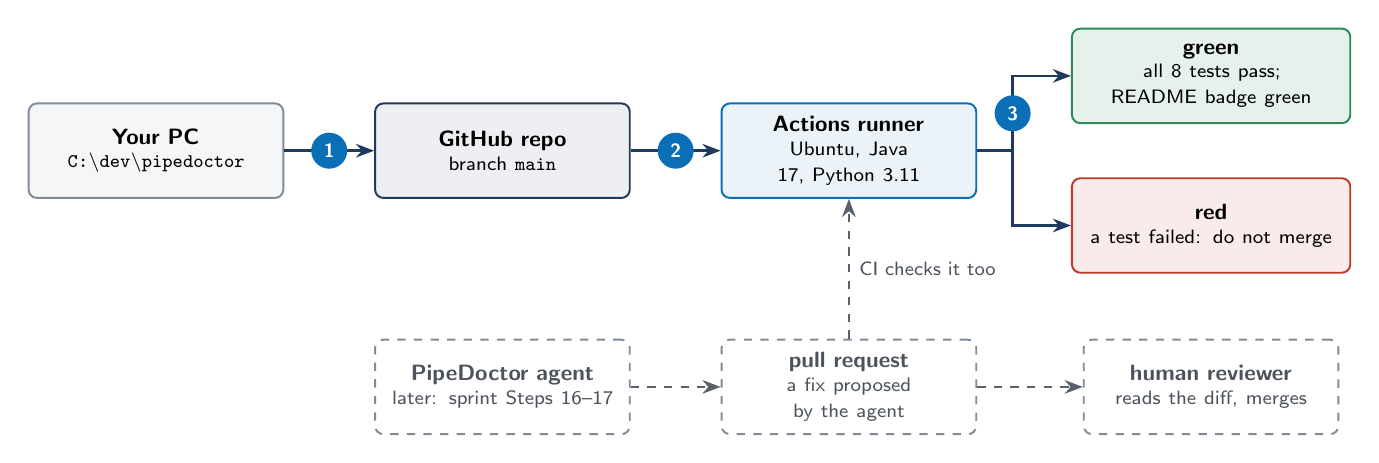
\begin{tikzpicture}[
  font=\footnotesize,
  box/.style={draw=navy,rounded corners=3pt,fill=white,minimum height=1.2cm,text width=3.0cm,align=center,line width=0.7pt},
  pc/.style={box,draw=silver,fill=rowgray},
  gh/.style={box,draw=navy,fill=navy!8},
  run/.style={box,draw=azure,fill=azure!8},
  okn/.style={box,draw=ok,fill=ok!12,text width=3.3cm},
  bad/.style={box,draw=alert,fill=alert!10,text width=3.3cm},
  fut/.style={box,draw=silver,dashed,fill=white,text=silver!60!black},
  arr/.style={-{Stealth[length=2.3mm]},line width=0.9pt,color=navy},
  bd/.style={circle,fill=azure,text=white,inner sep=0pt,minimum size=13pt,font=\bfseries\scriptsize}
]
\node[pc]  (pc)  at (0,0)     {\textbf{Your PC}\\[-1pt]\scriptsize\texttt{C:\textbackslash dev\textbackslash pipedoctor}};
\node[gh]  (gh)  at (4.4,0)   {\textbf{GitHub repo}\\[-1pt]\scriptsize branch \texttt{main}};
\node[run] (rn)  at (8.8,0)   {\textbf{Actions runner}\\[-1pt]\scriptsize Ubuntu, Java 17, Python 3.11};
\node[okn] (ok)  at (13.4,0.95)  {\textbf{green}\\[-1pt]\scriptsize all 8 tests pass; README badge green};
\node[bad] (ko)  at (13.4,-0.95) {\textbf{red}\\[-1pt]\scriptsize a test failed: do not merge};
\draw[arr] (pc) -- node[bd] {1} (gh);
\draw[arr] (gh) -- node[bd] {2} (rn);
\draw[arr] (rn.east) -- ++(0.45,0) |- node[bd,pos=0.25] {3} (ok.west);
\draw[arr] (rn.east) -- ++(0.45,0) |- (ko.west);
\node[fut] (ag) at (4.4,-3.0) {\textbf{PipeDoctor agent}\\[-1pt]\scriptsize later: sprint Steps 16--17};
\node[fut] (pr) at (8.8,-3.0) {\textbf{pull request}\\[-1pt]\scriptsize a fix proposed by the agent};
\node[fut] (hu) at (13.4,-3.0) {\textbf{human reviewer}\\[-1pt]\scriptsize reads the diff, merges};
\draw[arr,dashed,color=silver!70!black] (ag) -- (pr);
\draw[arr,dashed,color=silver!70!black] (pr) -- node[right,font=\scriptsize,text=silver!60!black] {CI checks it too} (rn.south);
\draw[arr,dashed,color=silver!70!black] (pr) -- (hu);
\end{tikzpicture}
\figcap{\textbf{Figure 1.} \badge{1} \texttt{git push} \quad \badge{2} the push triggers \f{ci.yml} \quad \badge{3} the runner reports a result. Dashed grey = what comes later: the agent's pull requests go through the same CI.}
\end{figure}

\section{The files I added}
\subsection*{\f{.github/workflows/ci.yml} \textemdash\ the CI recipe}
\rowcolors{2}{rowgray}{white}
\begin{tabularx}{\textwidth}{@{}>{\ttfamily\footnotesize}p{1.6cm}X@{}}
\toprule
Lines & What they say \\
\midrule
3--6 & Run on every push to \texttt{main} and on every pull request. The second part matters later: the agent's PRs get tested before a human looks at them. \\
8--9 & \texttt{permissions: contents: read}. The job can read the code and nothing else (least privilege, the same idea as PipeDoctor's guardrails). \\
11--13 & If you push twice quickly, cancel the older run on the same branch. \\
16--19 & One job on a fresh \texttt{ubuntu-latest} machine, stopped after 15 minutes if stuck. \\
21 & \texttt{actions/checkout}: download your code onto the runner. \\
24--27 & Install Java 17 (Temurin). Spark needs the JVM, exactly like \f{docker/Dockerfile} line 5. \\
29--33 & Install Python 3.11; pip downloads are cached, keyed on \f{docker/requirements.txt}. \\
35--36 & \texttt{pip install -r docker/requirements.txt}: the \emph{same pinned versions} as the Docker image (PySpark 3.5.3, Delta 3.2.1, pytest 8.3.3). \\
39--42 & Run \texttt{python -m pytest pipelines/tests -q}, the same test command as on your PC. \\
\bottomrule
\end{tabularx}

\medskip
\textbf{Why the runner does not build the Docker image.} It would add about 2.5 minutes for no gain: the tests use plain Spark without Delta (\f{pipelines/tests/conftest.py:8}), and the dependency versions are pinned to the same numbers. The cost is a small risk of drift between the two environments; we accept it and will revisit it in sprint Step 26.

\subsection*{\f{.gitattributes} and \f{.gitignore}}
\begin{itemize}[leftmargin=14pt,itemsep=2pt]
\item \f{.gitattributes}: \texttt{* text=auto eol=lf} keeps Unix line endings. Windows would otherwise write CRLF, which breaks shell scripts inside Docker. You may see the warning \texttt{LF will be replaced by CRLF} on Windows; it is harmless.
\item \f{.gitignore} (already there): excludes \f{data/}, \f{spark-warehouse/}, \f{.env}, Terraform state. The 1.3\,GB of data never goes to GitHub; anyone can recreate it with \f{scripts/download_taxi_data.py}.
\end{itemize}

\subsection*{Decision D12 (\f{docs/decision-log.md})}
Repository \texttt{Aymannel04/pipedoctor}, \textbf{private} until the release (Gate 4), because \f{docs/} holds interview material and drafts. GitHub Actions allows enough free minutes on private repositories for unit tests. At the release we review \f{docs/} and make it public: a public repository is the real portfolio piece.

\section{What you run, in order}
Open \textbf{PowerShell}. Lines starting with \texttt{\#} are comments.

\subsection*{A. Copy the project out of OneDrive}
\begin{lstlisting}[style=cmd]
# close VS Code and any running Docker command first
mkdir C:\dev
robocopy "C:\Users\Ayman\OneDrive\Desktop\Pipe Doctor\pipedoctor" C:\dev\pipedoctor /E /XD spark-warehouse .pytest_cache __pycache__ /XF *.pyc
cd C:\dev\pipedoctor
code .
\end{lstlisting}
\texttt{robocopy} reports success with exit codes 0 to 7; only 8 or more means an error. The copy includes \f{data/}, so you do not need to download or rebuild anything. Keep the OneDrive copy for now as a backup.

\subsection*{B. Create the local repository}
\begin{lstlisting}[style=cmd]
git init -b main
git config user.name "Ayman"
git config user.email "YOUR-GITHUB-EMAIL"
git add .
git status
\end{lstlisting}
\textbf{Check the \texttt{git status} output before committing:} it must list \f{pipelines/}, \f{docs/}, \f{docker/}, \f{.github/}, and must \emph{not} list \f{data/}. If \f{data/} appears, stop and show me.
\begin{lstlisting}[style=cmd]
git commit -m "Steps 1-3: project skeleton, local lakehouse, CI"
\end{lstlisting}

\subsection*{C. Create the empty repository on GitHub}
In the browser: \url{https://github.com/new}. Owner \texttt{Aymannel04}, name \texttt{pipedoctor}, \textbf{Private}, and leave \emph{all} the ``initialise with'' boxes unticked (no README, no \texttt{.gitignore}, no licence), otherwise the first push conflicts.

\subsection*{D. Push}
\begin{lstlisting}[style=cmd]
git remote add origin https://github.com/Aymannel04/pipedoctor.git
git push -u origin main
\end{lstlisting}
Git for Windows opens a browser window to log in to GitHub the first time; accept it.

\subsection*{E. Watch the CI}
Open \url{https://github.com/Aymannel04/pipedoctor/actions}. The workflow \texttt{CI} starts by itself. Expect 2 to 4 minutes (the first run downloads 317\,MB of PySpark). A green tick means the tests pass on a clean machine.

\section{Checklist and what to send me}
\begin{itemize}[leftmargin=14pt,itemsep=2pt]
\item[\fbox{\phantom{x}}] \texttt{git status} did not list \f{data/}.
\item[\fbox{\phantom{x}}] \texttt{git push} finished without error.
\item[\fbox{\phantom{x}}] The Actions tab shows a green \texttt{CI} run. \textbf{Send me a screenshot or the status (green or red).}
\item[\fbox{\phantom{x}}] Open the repository page: the README shows the architecture picture.
\end{itemize}

\Needspace*{16\baselineskip}
\section{If something goes wrong}
\rowcolors{2}{rowgray}{white}
\begin{tabularx}{\textwidth}{@{}p{5.4cm}X@{}}
\toprule
Symptom & Cause and fix \\
\midrule
\texttt{fatal: detected dubious ownership} & Git distrusts the folder owner. Run the \texttt{git config --global --add safe.directory} command that the message prints. \\
\texttt{remote: Repository not found} on push & The GitHub repository was not created yet, or the name differs. Check step C. \\
\texttt{rejected ... fetch first} & You ticked ``add a README'' on GitHub. Delete the repository, recreate it empty. \\
Push is very slow or huge & \f{data/} got added. Run \texttt{git rm -r --cached data} then amend the commit. \\
CI is red on the \emph{first} run & Read the log in the Actions tab. This is real practice: it is the same kind of log PipeDoctor will read. Paste the last 30 lines to me. \\
\texttt{LF will be replaced by CRLF} & Harmless warning, see \f{.gitattributes}. \\
\bottomrule
\end{tabularx}

\section{After this step}
Once CI is green, delete the \f{data/} folder inside the OneDrive copy to stop the sync. From then on we work in \f{C:\dev\pipedoctor}; I will ask for access to that folder so I can keep writing files there. Next is \textbf{sprint Step 4}: an Airflow DAG that runs the pipeline and writes a failure event when it breaks.

\end{document}
